\documentclass{article}
\usepackage[utf8]{inputenc}
\usepackage{graphicx}
\title{GitNotes}
\author{Charlie Jung}
\thanks{Kalid Azad from https://betterexplained.com/articles/a-visual-guide-to-version-control/ }
\date{\today}

\begin{document}

\maketitle
\newpage
\begin{flushedleft}

\underline{Version Control:} \\
\par

A good \textbf{VCS} has these elements: \\
\par

\textbf{Backup and Restore:} Files are saved as they are edited \par
Need a file from May 27, 2018? No problem! \\
\par

\textbf{Synchronization:} People can share files and stay up-to-date with the latest version \\
\par

\textbf{Short-Term Undo:} Throw away your changes? \par
You can go back immediately to the last \textit{stable} version \\
\par

\textbf{Long-Term Undo:} Go back to a project a year ago to fix a \underline{bug} \\
\par

\textbf{Track Changes:} As files are updated: you can leave messages ("commit messages") explaining why the change happened. (in VCS; not the file) \\
\par

\textbf{Track Ownership:} VCS tags every change to a user \\
\par

\textbf{Sandboxing:} Making a big change? Make temp changes in an isolated are anad test it out before checking in your changes. \\
\par

\textbf{Branching and Merging:} You can work on a new branch & merge later \\
\par

\textbf{\underline{Language and Technical Jargon:}} \\
\par

\textbf{Basic Actions:} \\
\par

\textbf{Add:} Put a file in the repository for the first time. \par
Begin Tracking with Version Control) \\
\par

\textbf{Revision:} What version a file is? (v1, v2, etc...) \\
\par

\textbf{Head:} Latest Revision in a repository \\
\par

\textbf{Check Out:} Download a file from a repository \\
\par

\textbf{Check In:} Upload a file to a repository. \par
File gets a new revision # and people can check the latest Revision out \\
\par

\textbf{Check In Message:}  A short message describing what has changed \\
\par

\textbf{Changelog/History:} A list of hcanges made to a file since it was created \\
\par

\textbf{Update/Sync:} Synchronize your \textbf{local files} with the latest from the repository. \par
This lets you grab all the latest revision of all the files \\
\par

\textbf{Revert:} Throw away your local changes and reload \par
the latest version from your repository \\
\par

\textbf{\underline{Advanced Actions:}} \\
\par

\textbf{Branch:} Create a separate copy of a file/folder for private use (bug fixing, testing) \par
Branch is both a verb ("Branch the code") and a noun ("Which branch is it in?) \\
\par

\textbf{Diff/Change/Delta:} Finding the difference between two files \\
\par

\textbf{Merge or Patch:} Apply changes from one file to another: Bring it up to date \\
\par

\textbf{Conflict:} When pending changes to a file contradict each other (both changes cannot be applied) \\
\par

\textbf{Resolve:} Fixing the changes that contradict each other and checking in the correct version \\
\par

\textbf{Locking:} Taking control of a file so nobody can edit it unless you unlock it \\
\par

\textbf{Breaking the Lock:} Forcibly unlocking a file so you can edit it \\
\par

\textbf{Check out for edit:} Checking out an "editable" version of a file \\
\par

\textbf{Check Ins:} \\
\par

Simple Scenario: \\
\par

Checking in a file (list.txt) and modifying it over time.

Basic Check  In:

\begin{figure}[htp]
\centering
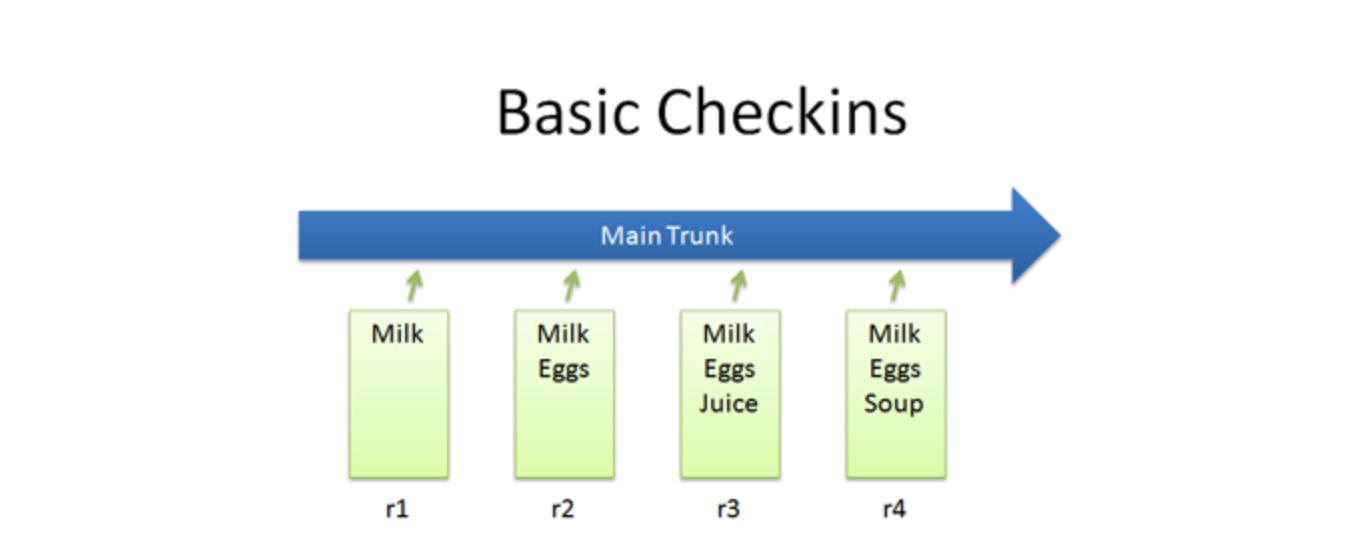
\includegraphics[width=4cm]{BasicCheckIn.png}
\caption{Basic Check In Diagram}
\label{fig:BCIDiagram}
\end{figure} 


\textbf{Subversion Example:} \\
\par

svn add list.txt \par

(modify the file)... \par

svn ci list.txt -m "Changed" \\
\par

\textbf{Checkout and Edit:} \\
\par

\begin{figure}[htp]
\centering
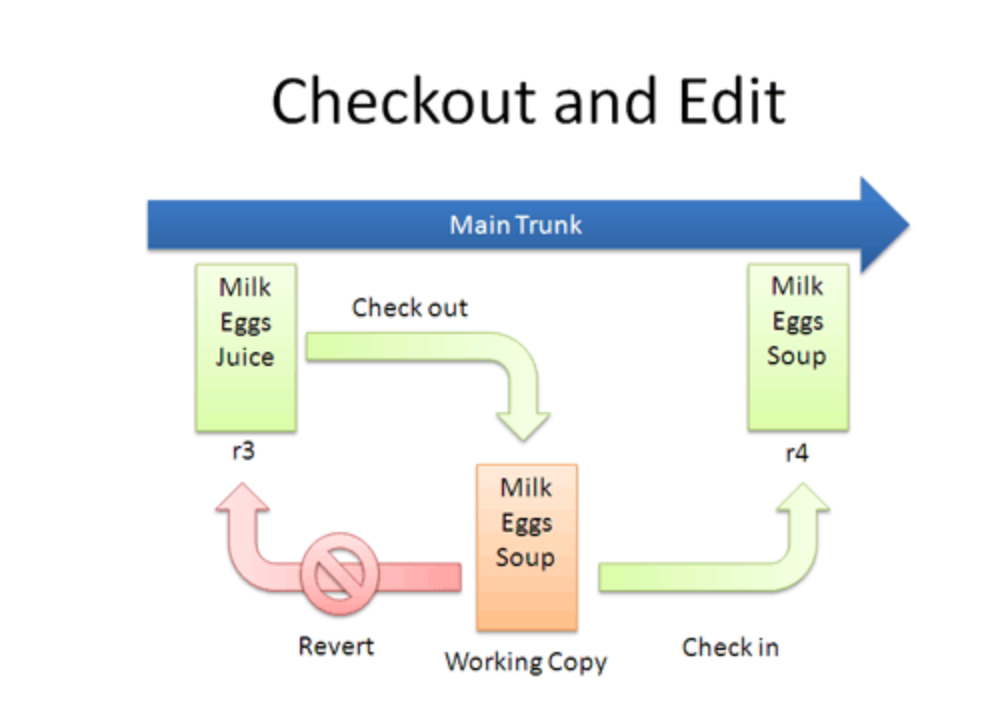
\includegraphics[width=4cm]{CheckOutAndEdit.png}
\caption{Basic Check Out and Edit Diagram}
\label{fig:BCOEDiagram}
\end{figure} 

\textbf{Subversion Commands:} \\
\par

svn co list.txt (get latest version) \par
... edit file ... \par
svn revert list.txt (throw away) \par
svn co -r2 list.txt (check out a particular revision) \\
\par

\textbf{Diffs:} \\
\par

\begin{figure}[htp]
\centering
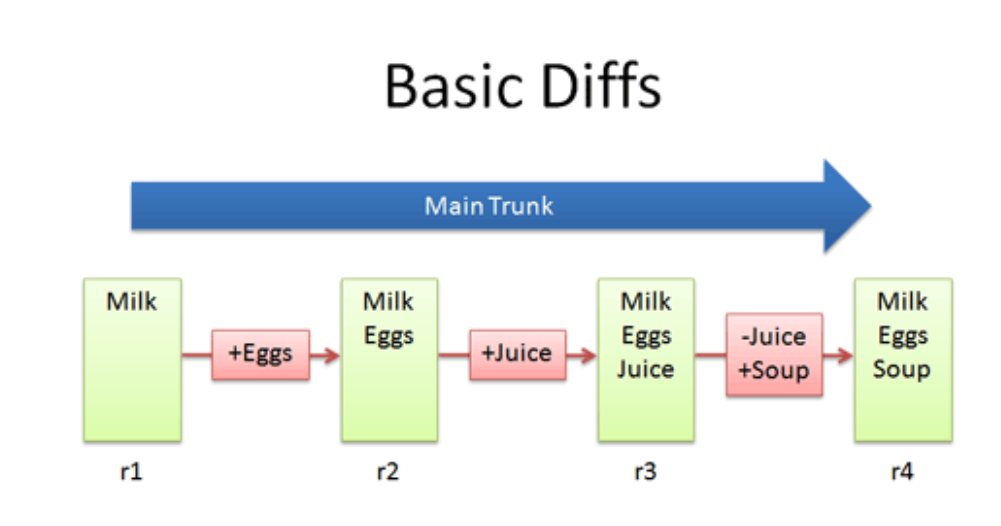
\includegraphics[width=4cm]{Diff.png}
\caption{Basic Differences Diagram}
\label{fig:BDDiagram}
\end{figure} 

Most VCS's store: src file and diffs

\underline{Subversion:} \\
\par

svn diff -r3:4 list.txt \\
\par

\textbf{Branching:} \\
\par

Branches let us copy code into a separate folder \\
\par

\begin{figure}[htp]
\centering
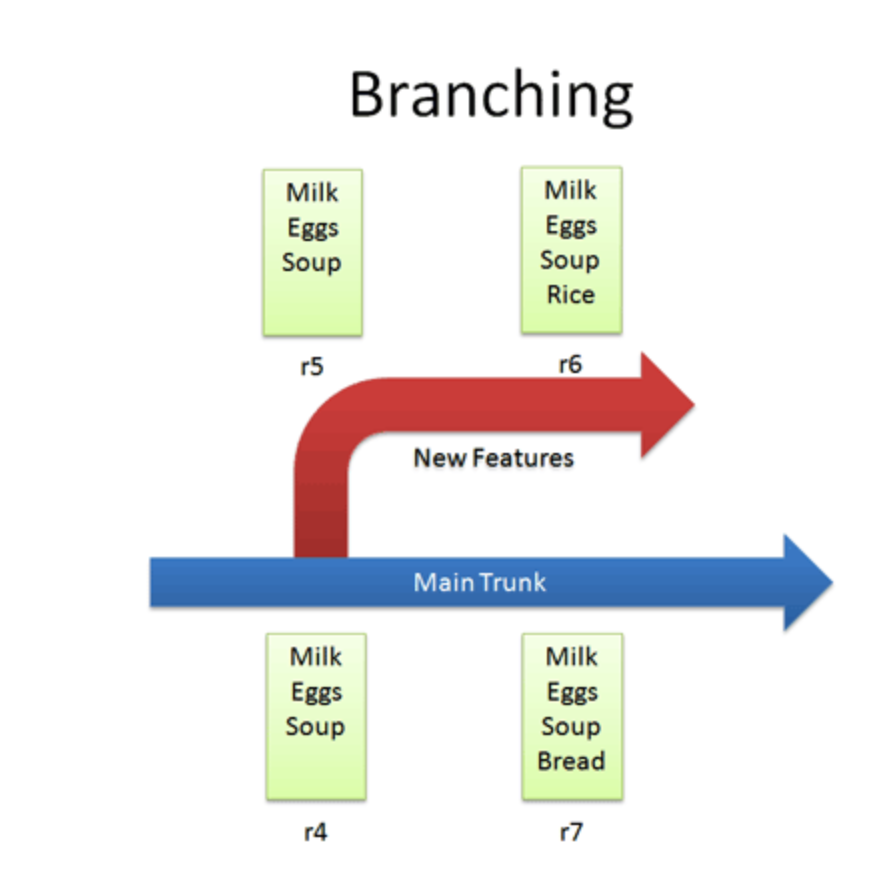
\includegraphics[width=4cm]{Branching.png}
\caption{Basic Branching Diagram}
\label{fig:BBDiagram}
\end{figure} 

\underline{In Subversion, you create a branch by copying a directory to another} \\
\par

svn copy http://path/to/trunk http://path/to/branch \\
\par

\textbf{Merging:} \\
\par

Let's say we wanted to get the "rice" feature from our experimental branch into the main line. How would we achieve this? \par
Diff r6 and r7 and apply that to the main line. \\
\par

Nope. We want to apply changes that happened in the specific (our case, experimental) branch. \par
We diff r5 \& r6 and apply it to the main trunk \\
\par

Diagram:


\begin{figure}[htp]
\centering
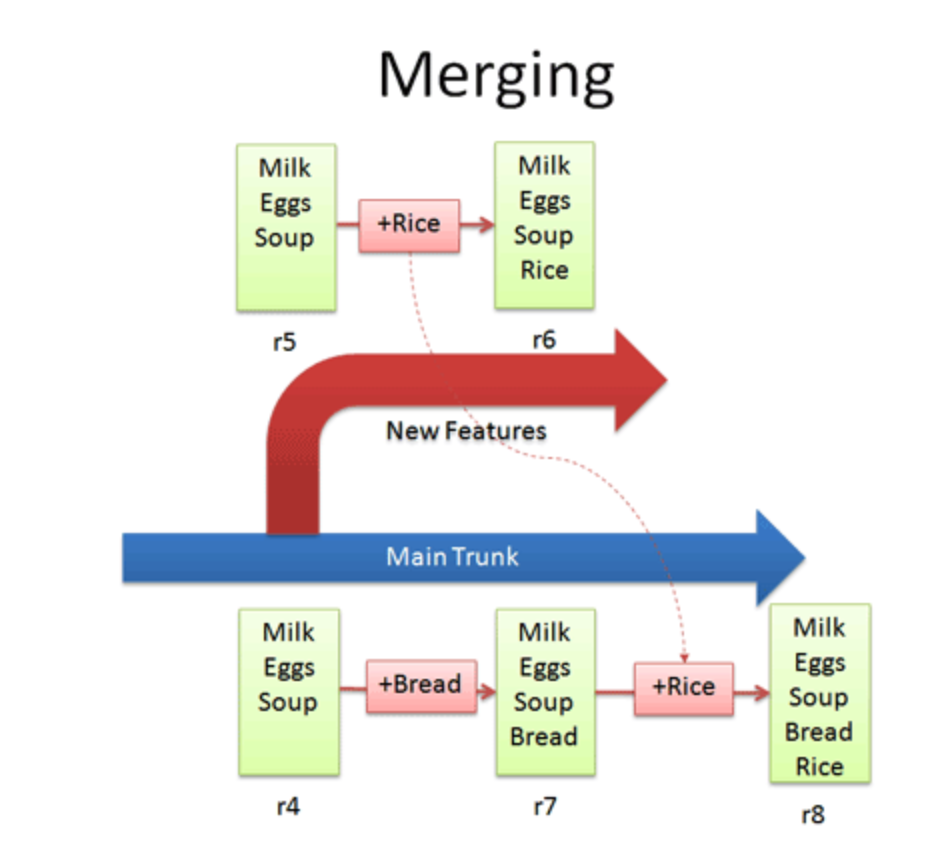
\includegraphics[width=4cm]{Merging.png}
\caption{Basic Merging Diagram}
\label{fig:BMDiagram}
\end{figure} 

\underline{In Subversion:} Merging is very close to diffing. \frame{Inside the main trunk:} \par
Run in SVN: \\
\par

svn merge -r5:6 http://path/to/branch \par
(Note: Subversion does not currently track what merges have been applied: If you are not careful, your changes could \par
be applied twice.) \\
\par

\underline{Current Advice:} Keep a changelog message reminding you that you have already merged r5 to r6 in \underline{main} \\
\par

\underline{Conflicts:} \\
\par

Many times, the VCS can automatically merge changes to different parts of a file. \par
\frame{Conflicts} can arise when changes don't sit well: \\
\par

Joe wants to remove eggs and replace it with cheese (-eggs, +cheese) \par
Sue wants to replace eggs with a hot dog (-eggs, +hotdogs) \\
\par

\underline{Conflicts} \\
\par


\begin{figure}[htp]
\centering
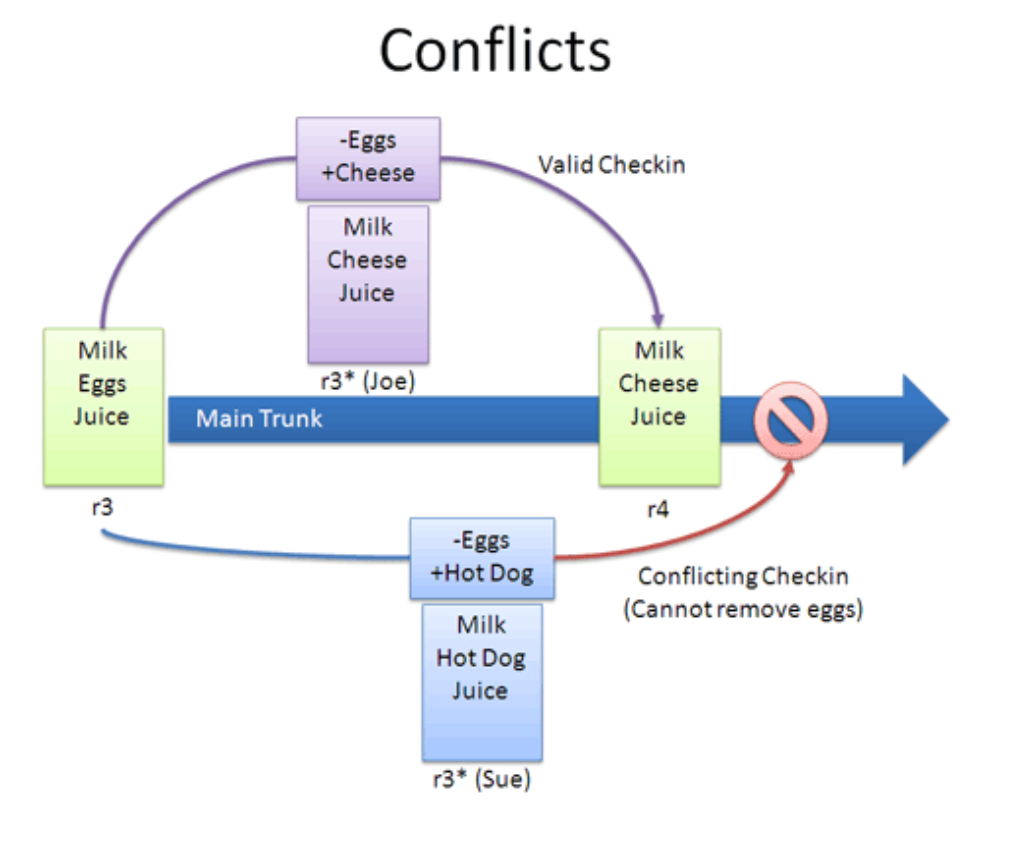
\includegraphics[width=4cm]{Conflicts.png}
\caption{Basic Conflicts Diagram}
\label{fig:BCDiagram}
\end{figure} 

The quicker check-in wins out: \\
\par

If VCS reports a conflict: \\
\par

\begin{itemize}
    \item Re-apply your changes
    \item Override old changes with your own changes
\end{itemize} \par
\par

\underline{Tagging:} \\
\par


\begin{figure}[htp]
\centering
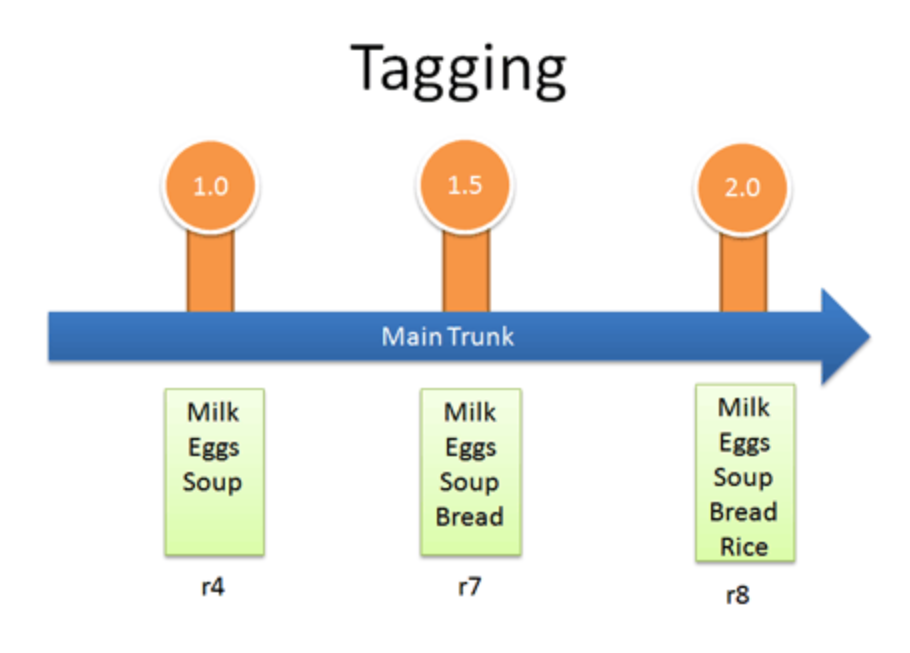
\includegraphics[width=4cm]{Tagging.png}
\caption{Basic Tagging Diagram}
\label{fig:BTDiagram}
\end{figure} 

(in trunk) \par
tags are named branches (non-editable) \par
svn copy to/revision to/tag \\
\par

Real Life Example: \par
MainLine \rightarrow Stable Windows \par
Each part (UI, Networking) has a unique branch \par

Reverse Integration: From branch \rightarrow trunk \\
\par

\textbf{Forward-Integrate:} Receive Latest Patches from main into their own branch ("pull") \\
\par

\textbf{Git Commands:} \\
\par

git clone \par
git config \par
git add \par
git status \par
git commit \par
git push \par
git pull \par
git branch \par
git checkout \par
git merge \\
\par

Branches are just pointers to \underline{commits} \\
\par













































\end{flushedleft}


\end{document}
